% Adjusting chapter title format for regular (numbered) chapters
\titleformat{\chapter}[display]
  {\normalfont\huge\bfseries\centering}{\chaptertitlename\ \thechapter}{20pt}{\Huge}

% Using similar styling for unnumbered chapters but without "Chapter" prefix
\titleformat{name=\chapter,numberless}
  {\normalfont\huge\bfseries\centering}{}{0pt}{\Huge}

\titlespacing*{\chapter}{0pt}{50pt}{40pt} % Adjust vertical spacing before and after the title

\chapter{Literature Review}
\label{chp:2}

To develop a comprehensive testing framework for DNNs, it is crucial to explore various domains that collectively contribute to this goal. This literature review aims to discuss the concepts of DNNs and AI systems, followed by an examination of the robustness of DNNs. Subsequently, the literature will be categorized into seven research modules: DNN testing framework, Specification, Sampling, Interpretability, Testcase Generation, Coverage Criteria and Error Summarization, each playing a vital role in the framework. 


\section{Deep Neural Networks and AI Systems}

DNNs mimic the structure of the human brain, consisting of millions of interconnected neurons. They extract high-level features from raw input using labeled training data without human interference.

Formally, a DNN is a function $f\colon\mathbb{R}^{s_0}\mapsto \mathbb{R}^{s_k}$ that takes as input a vector of size $s_0$ and produces a vector of size $s_k$. The function $f$ is computed by composing $k$ layers $L_1\colon\mathbb{R}^{s_0} \mapsto\mathbb{R}^{s_1}, \dots, L_k\colon\mathbb{R}^{s_{k-1}}\mapsto\mathbb{R}^{s_k}$ as $f(x) = L_k(\cdots L_2(L_1(x))\cdots)$.

Each layer~$L_i$ typically implements a non-linear function. For instance, a \emph{fully-connected} layer linearly transforms its input $x_{i-1}$ as $W x_{i-1} + b$, where $W\in\mathbb{R}^{s_{i} \times s_{i-1}}$ is the matrix of weights and $b\in\mathbb{R}^{s_i}$ is the bias vector. Then, it applies a non-linear activation function (e.g., sigmoid or rectified linear unit (ReLU)) component-wise, generating the output vector $x_i$. The weights specify how its input neurons are connected to its output neurons and are known as \emph{DNN parameters}. For more information about DNNs, we refer the reader to \cite{dnn_archi, Hassija, Liang}.

The objective of DNN training is to learn parameters during training to make accurate predictions on unseen data during real-world deployment.

When the prediction task is classification, then $s_k$ represents the number of classes. Assuming that $f(x) = (y_1,\dots,y_{s_k})$, the \emph{classification result} is $\displaystyle\mathop{\text{argmax}}_{i=1}^{s_k} y_i$, which is the index of the component with the highest probability $y_i$. By abuse of notation, sometimes we write $f(x)=c$ to denote the fact that $x$ was classified as $c$. We also write $f(x)_c$ to refer to $y_c$ which represents the probability of $x$ being in class $c$.

By an \emph{AI system}, we refer to any software system capable of performing complex tasks through the use of data, algorithms, and high computational power, which typically require human intelligence. These tasks include problem-solving, reasoning, decision-making, and natural language understanding.

Deep learning is a subset of AI that utilizes DNNs for complex pattern recognition. Some AI systems are solely based on DNN components, whereas \emph{hybrid} AI systems combine DNNs with traditional software to produce the final output.

\section{Robustness of Deep Neural Networks}

\begin{figure}[h]
  \centering
  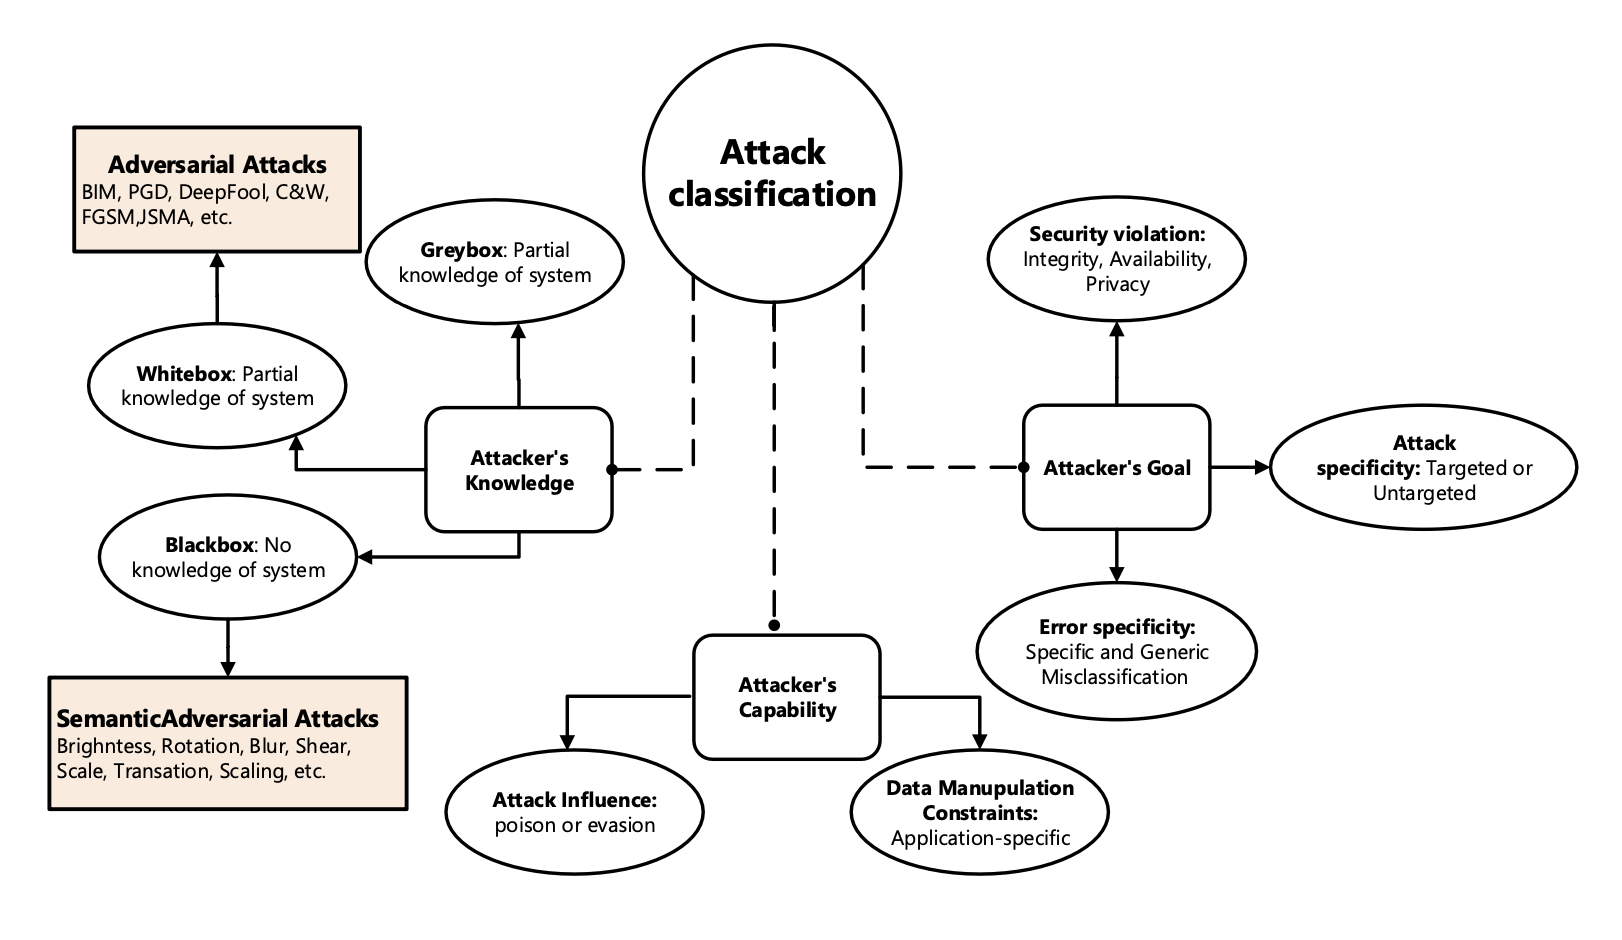
\includegraphics[width=\linewidth]{attackclassification.png}
  \caption{Attack classification}
  \label{fig:adv_threats}
\end{figure}


DNNs are known for their lack of robustness, which makes them vulnerable to adversarial attacks. Researchers have developed various attack techniques to expose these vulnerabilities by creating adversarial examples, which highlight the weaknesses of a DNN without providing any provable guarentee \cite{HuangX}. Fig. \ref{fig:adv_threats}  illustrates the different types of attack threats, emphasizing the complexity and variety of these attacks. Adversarial threats to DNNs can be understood through three main components: attacker's knowledge, attacker's goals, and attacker's capabilities \cite{Biggio}.
Attackers can have different levels of knowledge: white-box attacks have full knowledge of the DNN's architecture and parameters, gray-box attacks have partial knowledge, and black-box attacks have no knowledge and rely on input-output queries. The attacker's goals might include compromising the system's integrity, availability, or privacy, with attacks being either targeted (misclassifying specific inputs) or untargeted (causing general misclassification). Attackers can influence the model by poison attack \cite{poisonattack,Badnets} during training or evasion attack \cite{evasion} during testing, and these manipulations are often constrained by application-specific data alteration limits.\cite{Chakraborty}.



In the context of attacker's knowledge, different techniques are employed to create \emph{adversarial examples}. White-box attacks, such as Fast Gradient Sign Method (FGSM) \cite{FGSM}, Basic Iterative Method (BIM) \cite{BIM}, Carlini and Wagner (C\&W) Attack \cite{Carlini}, DeepFool \cite{deepfool}, and Jacobian-based Saliency Map Attack (JSMA) \cite{JSMA}. These techniques specifically manipulate input data to create slight perturbations that maximize the network prediction error, causing the DNN to make incorrect predictions \cite{Hosseini}.

Conversely, black-box attacks often involve \emph{semantic adversarial examples} \cite{HuangX,deeptest,Engstrom,Pei}, which are not limited to slight modifications of the image. These attacks can involve any transformation that preserves the semantics of the image, such as changes in brightness, contrast, shear, translation, scale, and rotations. These modifications, illustrated in Fig. \ref{fig:image-trans}, can significantly affect the DNN's performance. 



\begin{center}
  \fcolorbox{gray}{lightgray}{
  \parbox{0.95\linewidth}{
  \textbf{Note:} Currently, I have explored both black-box and white-box techniques to understand the differences between these adversarial examples. Further exploration is needed for grey-box techniques.

  }
  }
  \end{center}

  \begin{figure*}
    \centering
    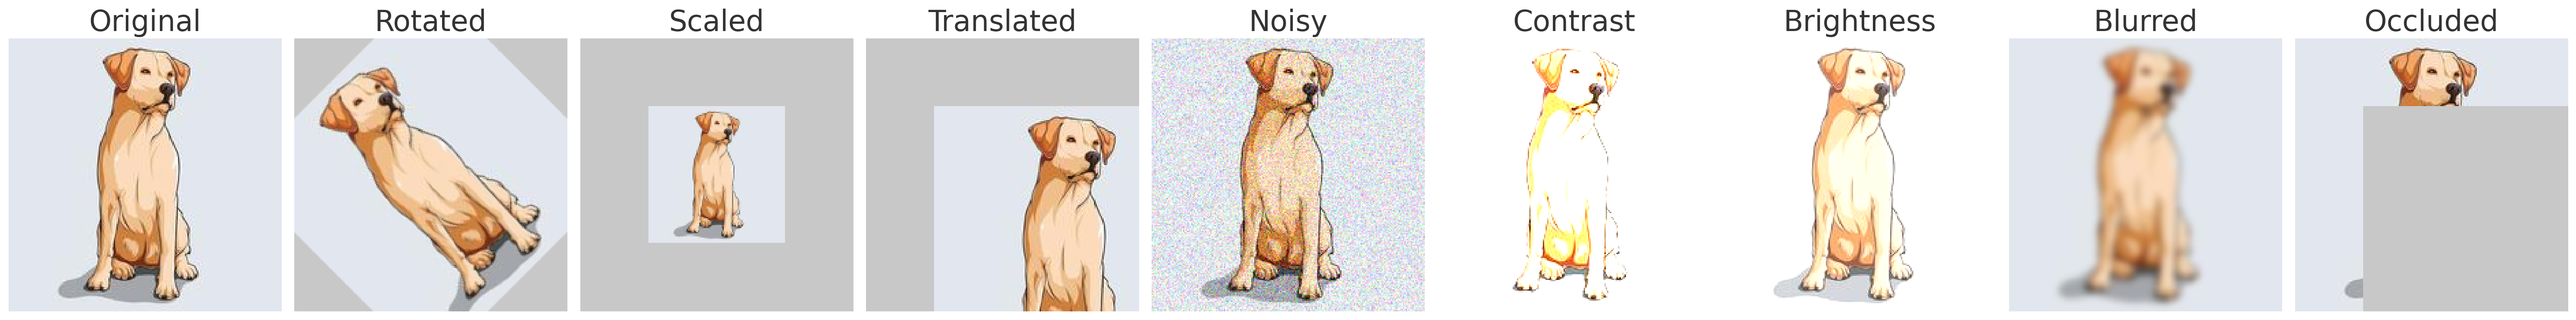
\includegraphics[width=\linewidth]{figures/output_update.png}
    \caption{Semantic Adversarial Examples}
    \label{fig:image-trans}
  \end{figure*}


\section{Research Modules}

I have categorized the literature work into seven research areas as shown in Figure \ref{fig:thematic_wheel}. 
\begin{figure*}[h]
  \centering
  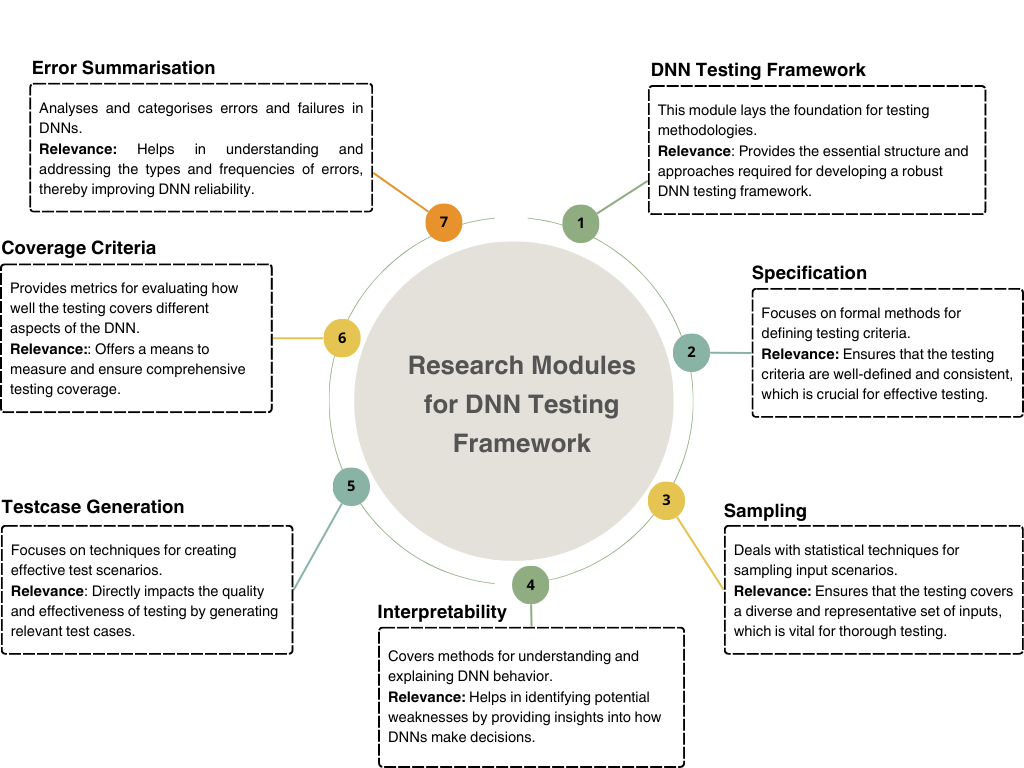
\includegraphics[width=\linewidth]{literaturedomains.png}
  \caption{Thematic Wheel Diagram of Research Modules for DNN Testing Framework}
  \label{fig:thematic_wheel}
\end{figure*}



 Various frameworks have been proposed in the literature, each incorporating different methodologies and components to address specific aspects of DNN testing. Table \ref{tab:Comprison of Research Modules} provides a comparison of several DNN testing frameworks based on their inclusion of key areas such as specification, sampling, interpretability, testcase generation, coverage criteria, and error summarization. It indicates that no single paper comprehensively addresses all the areas necessary for a robust DNN testing framework. Most research, such as \cite{deepxplore}, \cite{deeptest}, \cite{Wicker}, \cite{Ma}, \cite{SunY}, \cite{Sun}, \cite{Cheng}, \cite{Kim}, \cite{Concolic}, \cite{Deepconcolic}, \cite{tensorfuzz}, \cite{Deephunter}, \cite{DLFuzz}, \cite{Sayah}, and \cite{Dola}, focuses on testcase generation and coverage criteria, providing methods to generate effective test cases and evaluate DNNs. Notably, \cite{Braiek} reviews all the challenges of testing DNNs, discussing each area but without providing concrete solutions.

Building upon this foundational work, test-case generation methods are influenced by traditional software testing methods like fuzz testing, metamorphic testing, and symbolic execution. DeepXplore \cite{deepxplore} is a whitebox test-case generation method that checks how different DNNs behave using domain-specific rules on inputs. It uses multiple models trained on the same data to find differences in their prediction. It aims to jointly optimize neuron coverage and different predictions between models, using gradient ascent for test generation. DeepTest \cite{deeptest} focuses on generating test inputs for autonomous cars by applying domain-specific rules on seed inputs. It uses a greedy search method based on the NC metric to create effective test cases. Adapting traditional fuzzing techniques for DNN test-case generation includes methods like DLFuzz \cite{DLFuzz} and TensorFuzz \cite{tensorfuzz}. DLFuzz generates adversarial inputs based on neuron coverage, akin to DeepXplore, but does not require multiple models and uses constraints to keep new inputs similar to originals. TensorFuzz employs coverage-guided testing to uncover numerical issues and discrepancies in DNNs and their quantized versions. DeepConcolic \cite{Deepconcolic} employs a concolic testing approach to generate adversarial inputs for DNN testing. It combines symbolic execution with concrete execution path information to meet coverage criteria, supporting both NC and MC/DC criteria.

In traditional software testing, coverage criteria measure how thoroughly software is tested. In DNNs, coverage might not directly apply to lines of code but rather to the input space or the variety of data the model can effectively handle or provide predictions for. Neuron coverage (NC) \cite{deepxplore} is the first coverage metric proposed in the literature to test DNNs. It is defined as the ratio of neurons activated by a test input to the total number of neurons in the model, where a neuron is activated when its activation value exceeds a predefined threshold. Ma et al. \cite{Ma} proposed a variety of coverage metrics, including K-multisection neuron coverage (KMNC), Neuron boundary coverage (NBC), and Strong neuron activation coverage (SNAC). KMNC calculates coverage by dividing the interval between lower and upper bounds into k-bins and measuring the number of bins activated by the test inputs. NBC measures the ratio of corner case regions covered by test inputs, with corner cases defined as activation values below or above those observed during training. SNAC similarly measures how many upper corner cases, defined as activation values above the training range, are covered by test inputs. Modified Condition/Decision Coverage (MC/DC) \cite{SunY} captures causal changes in test inputs based on the sign and value change of a neuron's activation. Likelihood-based Surprise Adequacy (LSA) uses Kernel Density Estimation (KDE) to estimate the likelihood of a test input during the training phase, prioritizing inputs with higher LSA scores as they are closer to classification boundaries. Distance-based Surprise Adequacy (DSA) is an alternative to LSA that uses the distance between activation traces of new test inputs and those observed during training \cite{Kim}.

Efficient sampling methods, crucial for identifying representative input scenarios, have not been the primary focus of existing studies. Sampling is a crucial step in the testing of DNNs, as it involves selecting a representative subset of inputs from a potentially vast input space. Depending on the testing objectives, different sampling techniques can be employed to ensure comprehensive testing. Stratified sampling ensures that all groups (or strata) within the data are represented, which is particularly useful when the specification requires equal representation from all categories. This technique needs prior knowledge of the groups to be effective \cite{Stratifiedsampling}. When the focus is on identifying critical samples, techniques like Borderline-SMOTE, ADASYN, and NearMiss are particularly useful. Borderline-SMOTE generates synthetic examples near the class borders, targeting challenging areas and thus helping to identify corner cases. However, it can still introduce noise \cite{Han2005}. ADASYN (Adaptive Synthetic Sampling Approach for Imbalanced Learning) adjusts the number of synthetic samples generated for each minority class example according to its difficulty level, focusing more on difficult-to-learn examples but might also introduce noise \cite{He2008}. NearMiss focuses on selecting examples close to the decision boundary, emphasizing difficult examples, but may discard useful information \cite{near-miss}. By integrating these advanced sampling techniques into DNN testing frameworks, we can significantly enhance our ability to identify corner cases and ensure comprehensive coverage. Current research primarily focuses on generating effective input test cases through semantic adversarial examples or adversarial examples. However, it is crucial to first understand whether the samples selected for these test cases are optimal. By prioritizing the selection of high-quality samples, we can lay a stronger foundation for subsequent test case generation, leading to more reliable and insightful testing outcomes. This shift in focus could provide new directions for research and development in DNN testing, ensuring that the inputs used for test cases are truly representative and capable of revealing critical vulnerabilities.

Formal specification of testing requirements is another area that lacks attention in current research. Paper \cite{Scenic} introduces Scenic, a language specifically designed for scenario specification and scene generation, highlighting its utility in creating detailed and probabilistic environment models. While some papers on interpretability, such as \cite{Fidel, Lin, Walker, Rahnama, Watson, Kuppa} exist in the literature, they primarily focus on detecting adversarial examples rather than providing a comprehensive framework for DNN testing. Although interpretability is not a key component of my framework, it is an important area of research that I will use for test case generation. Additionally, error summarization is covered by even fewer papers like \cite{ChenJ} and \cite{Deepmutation}.

\begin{table*}[ht]
  \centering
  \renewcommand{\arraystretch}{1.5}
  \setlength{\tabcolsep}{8pt}
  \resizebox{\textwidth}{!}{
  \begin{tabular}{|>{\centering\arraybackslash}m{3.5cm}|>{\centering\arraybackslash}m{2.5cm}|>{\centering\arraybackslash}m{2.5cm}|>{\centering\arraybackslash}m{3cm}|>{\centering\arraybackslash}m{3.5cm}|>{\centering\arraybackslash}m{3.5cm}|>{\centering\arraybackslash}m{3.5cm}|}
  \hline
  \rowcolor[gray]{0.9} \textbf{Paper} & \textbf{Specification} & \textbf{Sampling} & \textbf{Interpretability} & \textbf{Testcase Generation} & \textbf{Coverage Criteria} & \textbf{Error Summarization} \\
  \hline
  ImprovedTesting\cite{Sekhon} & \tickNo & \tickNo & \tickNo & \tickYes & \tickYes & \tickNo \\
\hline
DeepXplore \cite{deepxplore} & \tickNo & \tickNo & \tickNo & \tickYes & \tickYes & \tickNo \\
  \hline
  Deeptest \cite{deeptest} & \tickNo & \tickNo & \tickNo & \tickYes & \tickYes & \tickNo \\
  \hline
  Feature-guided Testing \cite{Wicker}& \tickNo & \tickNo & \tickNo & \tickYes & \tickYes & \tickNo \\
\hline
DeepGauge \cite{Ma}& \tickNo & \tickNo & \tickNo & \tickYes & \tickYes & \tickNo \\
  \hline
  Testing DNNs \cite{SunY}& \tickNo & \tickNo & \tickNo & \tickYes & \tickYes & \tickNo \\
\hline
Structural Test Coverage \cite{Sun}& \tickNo & \tickNo & \tickNo & \tickYes & \tickYes & \tickNo \\
\hline

Quantitative Projection Coverage \cite{Cheng} & \tickNo & \tickNo & \tickNo & \tickYes & \tickYes & \tickNo \\
\hline
Surprise Adequacy \cite{Kim} & \tickNo & \tickNo & \tickNo & \tickYes & \tickYes & \tickNo \\
\hline
Concolic testing \cite{Concolic} & \tickNo & \tickNo & \tickNo & \tickYes & \tickYes & \tickNo \\
\hline
Deepconcolic \cite{Deepconcolic} & \tickNo & \tickNo & \tickNo & \tickYes & \tickYes & \tickNo \\
\hline
Tensorfuzz \cite{tensorfuzz} & \tickNo & \tickNo & \tickNo & \tickYes & \tickYes & \tickNo \\
\hline
Deephunter \cite{Deephunter} & \tickNo & \tickNo & \tickNo & \tickYes & \tickYes & \tickNo \\
\hline
DLFuzz \cite{DLFuzz} & \tickNo & \tickNo & \tickNo & \tickYes & \tickYes & \tickNo \\
\hline
Symbolic execution\cite{Gopinath} & \tickNo & \tickNo & \tickNo & \tickYes & \tickNo & \tickNo \\
\hline
Automated Test Generation\cite{Agarwal} & \tickNo & \tickNo & \tickNo & \tickYes & \tickNo & \tickNo \\
\hline
DeepRoad \cite{Zhang} & \tickNo & \tickNo & \tickNo & \tickYes & \tickNo & \tickNo \\
\hline
MODE \cite{MODE} & \tickNo & \tickNo & \tickNo & \tickYes & \tickNo & \tickNo \\
\hline
Deepmutation \cite{Deepmutation} & \tickNo & \tickNo & \tickNo & \tickYes & \tickYes & \tickYes \\
% \hline
% \cite{Braiek} & \tickYes & \tickYes & \tickYes & \tickYes & \tickYes & \tickYes \\
\hline
Distribution-aware testing \cite{Dola} & \tickNo & \tickNo & \tickNo & \tickYes & \tickYes & \tickNo \\
\hline
Robustness testing \cite{Sayah} & \tickNo & \tickNo & \tickNo & \tickYes & \tickYes & \tickNo \\
\hline
Understanding Framework Bugs\cite{ChenJ} & \tickNo & \tickNo & \tickNo & \tickYes & \tickYes & \tickYes \\
\hline
%Specification
Scenic\cite{Scenic} & \tickYes & \tickNo & \tickNo & \tickNo & \tickNo & \tickNo \\
\hline
% SHAP
SHAP signatures\cite{Fidel} & \tickNo & \tickNo & \tickYes & \tickNo & \tickNo & \tickNo \\
\hline
DeepSHAP \cite{Lin} & \tickNo & \tickNo & \tickYes & \tickNo & \tickNo & \tickNo \\
\hline
Attribution Analysis \cite{Walker} & \tickNo & \tickNo & \tickYes & \tickNo & \tickNo & \tickNo \\
\hline
Adversarial Explaining \cite{Rahnama} & \tickNo & \tickNo & \tickYes & \tickNo & \tickNo & \tickNo \\
\hline
Attack-Agnostic Detection\cite{Watson} & \tickNo & \tickNo & \tickYes & \tickNo & \tickNo & \tickNo \\
\hline
XAI\cite{Kuppa} & \tickNo & \tickNo & \tickYes & \tickNo & \tickNo & \tickNo \\
\hline
%sampling
Stratified sampling\cite{Stratifiedsampling} & \tickNo & \tickYes & \tickNo & \tickNo & \tickNo & \tickNo \\
\hline
Borderline-SMOTE \cite{Han2005} & \tickNo & \tickYes & \tickNo & \tickNo & \tickNo & \tickNo \\
\hline
ADASYN\cite{He2008} & \tickNo & \tickYes & \tickNo & \tickNo & \tickNo & \tickNo \\
\hline
Near-Miss\cite{near-miss} & \tickNo & \tickYes & \tickNo & \tickNo & \tickNo & \tickNo \\
\hline
  \end{tabular}
  }
  \caption{Analysis of DNN Testing Frameworks by Research Modules}
  \label{tab:Comprison of Research Modules}
  \end{table*}





% \section{Probabilistic Logic Programming (PLP)}

% Probabilistic Logic Programming (PLP) integrates probabilistic reasoning with the flexibility and expressiveness of logic programming. Traditional logic programming paradigms are deterministic, where each statement is either true or false. However, real-world scenarios often involve inherent uncertainties which deterministic logic cannot adequately handle. PLP addresses this limitation by allowing the representation of uncertainties directly within the logic framework, thereby enabling more nuanced and accurate modeling of complex domains \cite{Sato2001, Kimmig2011}.

% PLP has been explored extensively in various domains, including artificial intelligence, bioinformatics, and robotics. Sato and Kameya's introduction of PRISM \cite{Sato1997} was a significant milestone, combining statistical modeling with logic programming. Subsequent work by Koller and Friedman \cite{Koller2009} on probabilistic graphical models further influenced PLP frameworks. Various approaches to PLP, such as Logic Programs with Annotated Disjunctions (LPADs) \cite{Vennekens2004}, ProbLog \cite{DeRaedt2007}, Probabilistic Horn Abduction (PHA) \cite{Poole1993}, Independent Choice Logic (ICL) \cite{Poole1997}, and PRISM \cite{Sato2001}, have been developed, each leveraging the distribution semantics introduced by Sato \cite{Sato2001}.

% Among these, ProbLog has gained prominence due to its simplicity and expressive power, making it a preferred choice for many applications \cite{Kimmig2011}. ProbLog extends a logic program with probabilistic facts, defining a probability distribution over possible worlds (sets of facts). The probability of a query is computed by marginalizing over the probabilities of the worlds where the query is true.

% The need for explainable AI (XAI) has become increasingly important, particularly in domains where decisions must be transparent and interpretable, such as medical diagnosis and finance. Various approaches to XAI emphasize model interpretability and the generation of comprehensible explanations for model predictions \cite{Arrieta2020}. PLP, with its ability to generate explanations as part of its reasoning process, fits well within the XAI paradigm. Vidal \cite{Vidal2023} proposes a novel approach where explanations in PLP are represented as programs generated from a given query through unfolding-like transformations. This approach preserves the causal structure of inferences and ensures minimality by excluding irrelevant information. Such explanations can be parameterized to hide uninteresting details, making them comprehensible to non-expert users.


% Despite the extensive research in PLP and its applications, its use in testing DNNs is still very new. DNNs are powerful but often act like "black boxes," making it hard to understand and trust their predictions. This thesis presents a new way to use PLP for testing DNNs, an area that has not been explored before.

% By using PLP, we can turn the probabilistic outputs  of DNNs into probabilistic facts and rules. This helps in reasoning about uncertainties in the model's predictions and generating clear explanations for each prediction. This approach makes it easier to understand why a model made a certain prediction, giving insights into the model’s decision-making process. PLP can also help in debugging DNNs by identifying and fixing inconsistencies or unexpected behaviors in the predictions. By examining the probabilistic rules and their explanations, we can find areas for improvement more effectively. Additionally, PLP allows us to simulate different scenarios by changing probabilistic facts, which is useful for testing how robust the DNNs are under various conditions. This innovative method opens up new opportunities for research and practical applications, making deep learning systems more transparent, reliable, and trustworthy.

